\documentclass{beamer}
\usepackage{natbib}
\usepackage{amsmath}
\usetheme{Madrid}
%\setbeamertemplate{caption}[numbered]
\setbeamertemplate{caption}{\raggedright\insertcaption\par}
\newcommand{\bs}[1]{\boldsymbol{#1}}
\newcommand{\info}{\mathcal{I}}
\setbeamertemplate{frametitle continuation}[from second][]
\usepackage{natbib}
\bibliographystyle{chicago}
\usefonttheme{professionalfonts}
\usepackage[space]{grffile}
\hypersetup{
	colorlinks,
	allcolors=.,
	urlcolor=blue,
}


\title[Gender Gaps]{Childhood environment and gender gaps in adulthood}

\author[Yulia Sidi]{{\footnotesize Yulia Sidi}}
%\institute[HSPH]{}
\institute[UConn]{Applied General Exam \\ 
Department of Statistics, University of Connecticut}
\date[January 14, 2019]{{\scriptsize January 14, 2019}}


% Let's get started
\begin{document}

\begin{frame}
\titlepage
\end{frame}

\AtBeginSection[]{\begin{frame}{Outline}
  \tableofcontents[hideallsubsections, currentsection]
\end{frame}}

% Section and subsections will appear in the presentation overview
% and table of contents.
\section{Background}

\begin{frame}{Background}

The following topics were assessed by researchers in the past:
 
 \begin{itemize}
 	\item Gender gaps in adulthood in terms of employment rates, wage levels, etc.
 	\item Gender gaps in childhood in terms of test scores, high school graduation, etc.  
 \end{itemize}

The current paper "Childhood environment and gender gaps in adulthood" by \cite{chetty2016childhood} combined these two topics by asking:


\begin{block}{}
	\centering
	What is the role of family characteristics and childhood environment in shaping gender gaps in adulthood?
\end{block}

\end{frame}

\begin{frame}{Background}
The paper presented here is part of \href{https://opportunityinsights.org/}{Opportunity Insights} project, whose mission is 
\begin{block}{}
	\centering
	"to develop scalable policy solutions that will empower families throughout the United States to rise out of poverty and achieve better life outcomes"
\end{block} 

\end{frame}


\section{Data}

\begin{frame}{Data}
Data:
\begin{itemize}
	\item De-identified database of tax returns in US from 1996-2012 (IRS Databank), which was originally used by \cite{chetty2014land}:
\end{itemize}
\vline \\
Population of interest:
\begin{itemize}
	\item Children born between 1980-82, who are US citizens as of 2013 (approximately 10M children).
	\item Children linked with parents when claimed as dependents.
	\item Children were evaluated at age 30 for adulthood outcomes.
\end{itemize}
\end{frame}

\begin{frame}{Data}
The following three datasets used in this paper are publicly available on this \href{https://opportunityinsights.org/}{website}:
\begin{itemize}
	\item \textbf{Childhood and Gender Gaps: Commuting Zone Employment Rates by Gender and Parent Income Quintile and Other Covariates}
	\item County Employment Rates by Gender and Parent Income Quintile and Other Covariates
	\item \textbf{National Employment Rates, Earnings, and Other Outcomes by Parent Percentile and Gender}
\end{itemize}
\end{frame}

\begin{frame}{Outcomes of interest}
Children:
\begin{itemize}
	\item Employment: based on presence of W-2 form.
	\item Earnings: sum of all the earnings reported on individual's W-2 form.
	\item College attendance: based on at least one 1098-T form filed by a college, when a child was 18-23 years old.
\end{itemize}
\vline \\
Parents:
\begin{itemize}
	\item Household income: mean pre-tax fimily income averaged over the 5 years from 1996-2000 {\scriptsize(1.2\% of children, whose parents have zero mean income in this time period were excluded)}.
\end{itemize}
\end{frame}


\section{Results}
\subsection{Gender Gaps by Parent Income}

\begin{frame}{Overall Gender Gaps in Employment - Replicated}
\begin{columns}
	
	\begin{column}{0.52\textwidth}
		\vspace{\topsep}
		\begin{figure}
			\vspace{-0.5cm}	
			\includegraphics[width=\columnwidth]{../fig1.pdf}
			\caption{{\scriptsize Children’s Employment Rates by Parent Income Percentile}}
		\end{figure}	
	\end{column}
	
	\begin{column}{0.4\textwidth}
		\vspace{-2.5cm}	
		\begin{itemize}
			\item For low income families, boys have lower employment rates than girls, while for moderate/high income families boys have higher employment rates than girls.
			\item This result is driven by children from single parent family (appear in the original paper).
		\end{itemize}
	\end{column}
	
\end{columns}
\end{frame}

\begin{frame}{Overall Gender Gaps in Income - Replicated}
\begin{columns}
	
	\begin{column}{0.52\textwidth}
		\vspace{\topsep}
		\begin{figure}
			\vspace{-0.5cm}	
			\includegraphics[width=\columnwidth]{../fig4b.pdf}
			\caption{{\scriptsize Children’s Income Percentile Rank (at age 30) by Parent Income Percentile}}
		\end{figure}	
	\end{column}
	
	\begin{column}{0.4\textwidth}
		\vspace{-2.5cm}
		\begin{itemize}
			\item Income percentile rank is defined as sum of wage earnings, unemployment income, disability income, and self-employment income.
			\item Gender gap in individual income percentile ranks is smaller for low income parents.
		\end{itemize}
	
	\end{column}
	
\end{columns}
\end{frame}

\begin{frame}{Overall Gender Gaps in College Attendance - Replicated}
\begin{columns}
	
	\begin{column}{0.52\textwidth}
		\vspace{\topsep}
		\begin{figure}
			\vspace{-0.5cm}	
			\includegraphics[width=\columnwidth]{../fig4c.pdf}
			\caption{{\scriptsize Children’s College Attendance Rates by Parent Income Percentile}}
		\end{figure}	
	\end{column}
	
	\begin{column}{0.4\textwidth}
		\vspace{-2.5cm}	
		\begin{itemize}
			\item Across the distribution of the parent's income, girls attend college at higher rates than boys. 
			\item This gender gap is more pronounced at the lower income parents and almost disappers for the high income parents.
		\end{itemize}
	\end{column}
	
\end{columns}
\end{frame}


\begin{frame}{Overall Gender Gaps in College Attendance - Model}
Gap in college attendance rates as a function of parent household income percentile (PHIP).\\

\begin{columns}
	
	\begin{column}{0.4\textwidth}
		\vspace{\topsep}
		\begin{figure}
			\vspace{-0.5cm}	
			\includegraphics[width=\columnwidth]{../college_gap.pdf}
			\caption{{\scriptsize Gap in College Attendance Rates by Parent Income Percentile}}
		\end{figure}	
	\end{column}
	
	\begin{column}{0.5\textwidth}
		\vspace{-1cm}
		\begin{block}{Model 1}
			$$Y_i = \alpha + \beta_1 PHIP_i  + \epsilon_i; \  i=1,\dots 100$$
			$$\epsilon_i \ iid \ N(0,\sigma^2)$$
		\end{block}
		\begin{block}{Model 2}
			$$Y_i = \alpha + \beta_1 PHIP_i + \beta_1 PHIP_i^2 +  \epsilon_i$$
			$$\epsilon_i \ iid \ N(0,\sigma^2)$$
		\end{block}
	\end{column}
\end{columns}
\end{frame}
	
\begin{frame}{Overall Gender Gaps in College Attendance - Model Selection and Fit}

\begin{columns}
	\begin{column}{0.4\textwidth}
	\vspace{\topsep}
	\begin{figure}
		\vspace{-0.5cm}	
		\includegraphics[width=\columnwidth]{../college_gap_m1.pdf}
		\caption{{\scriptsize Model 1: Residuals vs Fitted}}
	\end{figure}	
\end{column}

\begin{column}{0.4\textwidth}
	\vspace{\topsep}
\begin{figure}
	\vspace{-0.5cm}	
	\includegraphics[width=\columnwidth]{../college_gap_m2.pdf}
	\caption{{\scriptsize Model 2: Residuals vs Fitted}}
\end{figure}	
\end{column}
\end{columns}

F-test resulted in $pvalue<0.001$, suggesting we have enough evidence to believe that the squared term of PHIP needs to be included in the model.
\end{frame}

\begin{frame}{Overall Gender Gaps in College Attendance - Model Results}

\begin{table}[ht]
	\centering
	\begin{tabular}{lrrrr}
		\hline
		Coefficient & Estimate & Std & Statistic & Pvalue \\ 
		\hline
		$Intercept$ & $-15.77$ & $0.10$ & $-158.70$ & $<.001$ \\ 
		$PHIP$ & $-0.06511$ & $0.00454$ & $-14.34$ & $<.001$ \\ 
		$PHIP^2$ & $0.0021$ & $0.00004$ & $47.73$ & $<.001$ \\ 
		\hline
		$R^2= 0.9949$
	\end{tabular}
\end{table}



	\begin{figure}
	\centering
	\includegraphics[width=4cm]{../college_gap_m2_fitted.pdf}
	\caption{{\scriptsize Model 2: Fitted Model}}
\end{figure}	

\end{frame}

\subsection{Geographic Variation in Gender Gaps}

\begin{frame}{Geographic Variation in Gender Gaps}
\begin{block}{}
	\centering
	We saw variations in gender gaps as a function of parents income. \\
	The next question is: \\
	how these gaps vary based on where children grow up?
\end{block}

The rest of the analysis will be performed at the commuting zone (CZ) level. According to \cite{chetty2016childhood}: CZs are aggregations of counties based on commuting patterns that provide a natural definition of local labor markets.
 
\end{frame}

\begin{frame}{Illustrative Example of Geographic Variation - Replicated}
\begin{columns}
	
	\begin{column}{0.52\textwidth}
		\vspace{\topsep}
		\begin{figure}
		\vspace{-0.5cm}	
		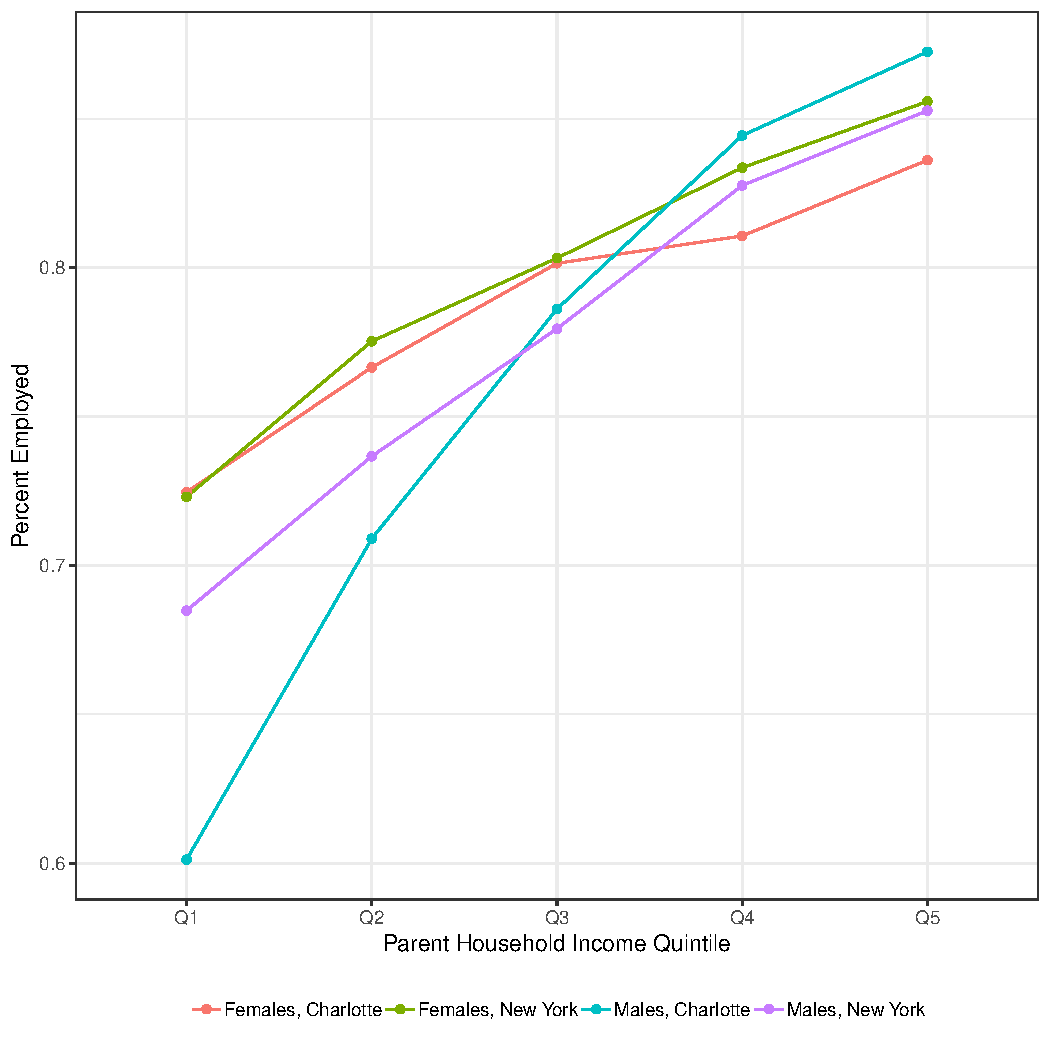
\includegraphics[width=\columnwidth]{../fig2.pdf}
		\caption{{\scriptsize Children’s Employment Rates by Gender and Parent Income Quintile:
			New York vs. Charlotte CZs}}
		\end{figure}	
\end{column}
	
	\begin{column}{0.4\textwidth}
				\vspace{-2.5cm}	
		\begin{itemize}
			\item Among females, percent employment is similar between the CZs across the distribution of parent household income.
			\item The gaps between females and males are more pronounced in Charlotte for low-income parents.
		\end{itemize}
	\end{column}
	
\end{columns}
\end{frame}


\begin{frame}{Illustrative Example of Geographic Variation}
\begin{columns}
	
	\begin{column}{0.52\textwidth}
		\vspace{\topsep}
		\begin{figure}
			\vspace{-0.5cm}	
			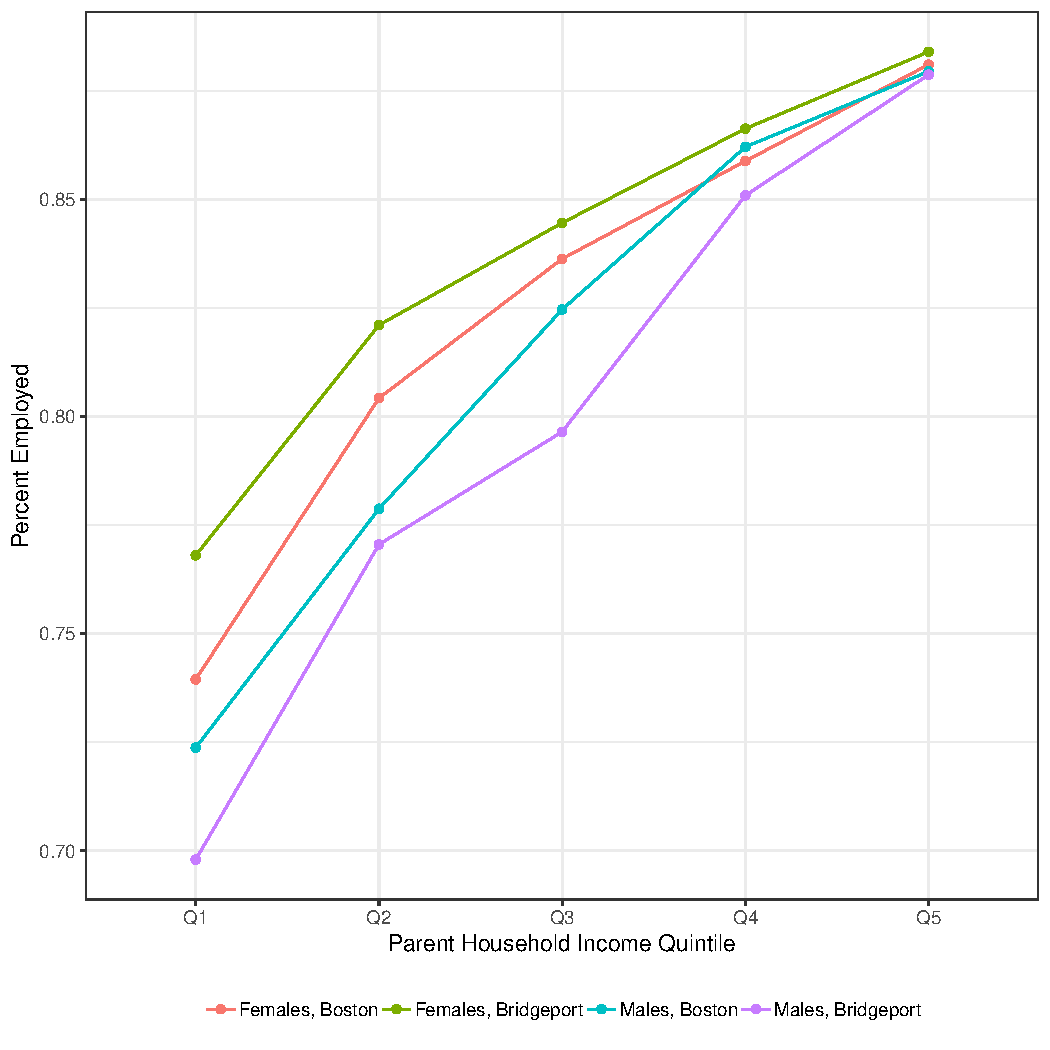
\includegraphics[width=\columnwidth]{../fig2_new.pdf}
			\caption{{\scriptsize Children’s Employment Rates by Gender and Parent Income Quintile:
					Boston vs. Bridgeport CZs}}
		\end{figure}	
	\end{column}
	
	\begin{column}{0.4\textwidth}
		\vspace{-2.5cm}	
		\begin{itemize}
			\item Among females, percent employment is slightly higher in Bridgeport across the parent income distribution. 
			\item The gaps between females and males are much more pronounced in Bridgeport for low/middle-income parents.
		\end{itemize}
	\end{column}
	
\end{columns}
\end{frame}

\begin{frame}{Illustrative Example of Geographic Variation}
\begin{columns}
	
	\begin{column}{0.52\textwidth}
		\vspace{\topsep}
		\begin{figure}
			\vspace{-0.5cm}	
			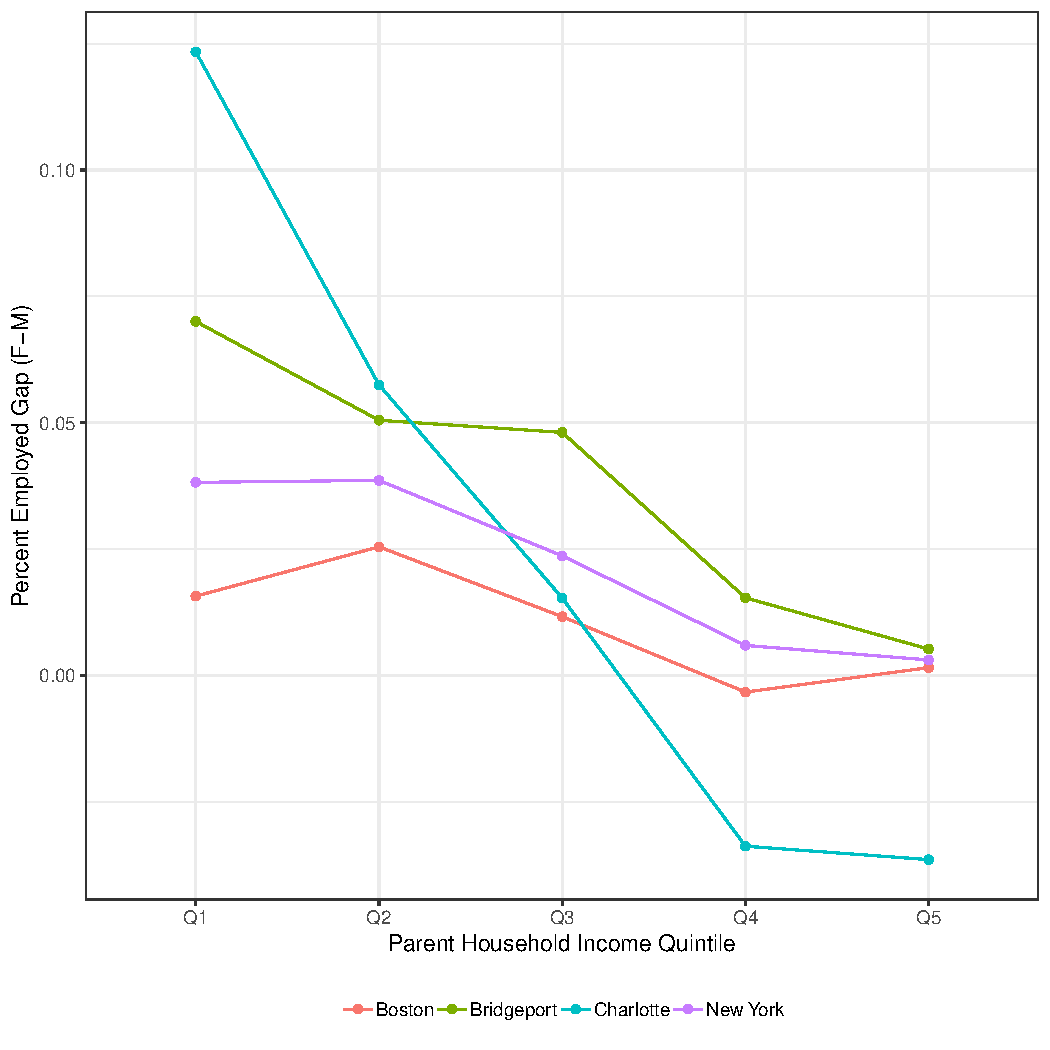
\includegraphics[width=\columnwidth]{../fig_ys.pdf}
			\caption{{\scriptsize Gender Gaps in Children’s Employment Rates by Parent Income Quintile:
					New-York/Charlotte/Boston/Bridgeport CZs}}
		\end{figure}	
	\end{column}
	
	\begin{column}{0.4\textwidth}
		\vspace{-2.5cm}	
		\begin{itemize}
			\item The gender gaps change more extremely in Charlotte. 
			\item In Boston, New-York and Bridgeport the gaps disappear with higher parent income, which is not the case for Charlotte.
		\end{itemize}
	\end{column}
	
\end{columns}
\end{frame}
\begin{frame}{Geographic Variation in Gender Gaps}

\begin{table}[ht]
	\centering
	\caption{Mean* Individual Income Ranks by Gender and Region}
	\begin{tabular}{lrrr}
		\hline
		Region & Males & Females & Gap \\ 
		\hline
		Midwest & 46.31 & 42.37 & 3.93 \\ 
		Northeast & 48.24 & 47.02 & 1.22 \\ 
		South & 43.63 & 41.11 & 2.52 \\ 
		West & 48.28 & 44.23 & 4.05 \\ 
		\hline
	\end{tabular}
\end{table}

Mean individual income ranks are defined at age 26 for children with parents at the 25th percentile of the national income distribution.\\
\vline\\
The gap in mean individual income ranks vary by region.\\
\vline\\
{\tiny * Means presented here are weighted by the population size at year 2000.}

\end{frame}


\begin{frame}{Geographic Variation in Gender Gaps}
\begin{block}{}
	\centering The illustrative examples shown above along with individual income ranks by regions suggest that gender gaps in low-income families vary geographically. 
\end{block}
\begin{block}{}
	\centering
	Next we will explore what characteristics of the areas where children grow up shape the gender gaps seen in the adulthood for children from low-income families.
\end{block}
\end{frame}

\begin{frame}
Missing values for the mean individual income ranks were 7\% and 7.6\% for males and females respectively.
\end{frame}


\begin{frame}{Gender Gaps in Mean Income Rank- Replicated}


\begin{table}[ht]
	\centering
	\caption{Male-Female Difference in Mean Income Rank}
	\footnotesize
	\begin{tabular}{lrrrr}
		\hline
		Covariate & Estimate & Std  & 95\% CI Lower & 95\% CI Upper \\ 
		\hline
		Segregation of Poverty & $-2.231$ & $0.186$ & $-2.604$ & $-1.858$ \\ 
		\% Black & $-1.820$ & $0.449$ &  $-2.722$ & $-0.918$ \\ 
		\% Single Mothers & $0.288$ &  $0.736$ & $-0.498$ & $1.075$ \\ 
		\hline
	\end{tabular}
\end{table}
$$Y_{ij}= \alpha + \beta_{seg(i)}Seg_{j(i)} + \beta_{blk(i)}Blk_{j(i)} + \beta_{sgl(i)}Slg_{j(i)} + State_i + \epsilon_{(i)j} $$
where $i=1,\dots ,51$ represents one of the states (including District of Columbia). $j$ varied between 1-64.\\

CZs are clustered/nested withing a specific state $\Rightarrow$  the nested model. Thus $\epsilon_{(i)j}$  are assumed to have Normal distribution with covariance structure that takes into account the nested design together with the population weights per CZ. State effects were set as fixed effects.

\end{frame}

\begin{frame}{Gender Gaps in Mean Income Rank- MICE}


\begin{table}[ht]
	\centering
	\caption{Male-Female Difference in Mean Income Rank-MICE}
	\footnotesize
	\begin{tabular}{lrrrr}
		\hline
		Covariate & Estimate & Std  & 95\% CI Lower & 95\% CI Upper \\ 
		\hline
		Segregation of Poverty & $-2.23$ & $0.18$  & $-2.59$ & $-1.87$ \\ 
		\% Black & $-1.816$ & $0.446$ &  $-2.69$ & $-1.867$ \\ 
		\% Single Mothers & $0.28$ &  $0.389$ & $-0.481$ & $1.043$ \\ 
		\hline
	\end{tabular}
\end{table}
This analysis was done using predictive mean matching for clustered design with weights \citep{vink2015partioned}.\\
 10 imputed datasets were used for this multiple imputation.

\end{frame}

\begin{frame}[allowframebreaks]
\frametitle<presentation>{References}
% This prints the bibliography on the slide
\tiny{\bibliography{applied_ref}}
\end{frame}

\begin{frame}
\begin{center}
\huge{Thank you!}
\end{center}
\end{frame}

\begin{frame}{Missing values in covariates}
\begin{table}[ht]
	\centering
	\tiny
	\begin{tabular}{lr}
		\hline
		Covariate & \% Missing \\ 
		\hline
		College tuition & 21.70 \\ 
		College Graduation Rate & 21.60 \\ 
		Number of Colleges per Capita & 21.2 \\ 
		High School Dropout Rate & 20 \\  
		Test Score Percentile & 4.9 \\ 
		Teenage (14-16) Labor Force Participation & 4.3 \\ 
		Top 1\% Income Share & 4.3 \\ 
		Student Teacher Ratio & 4 \\ 
		Violent Crime Rate & 3.6 \\ 
		Growth in Chinese Imports & 2.6 \\ 
		Social Capital Index & 2.6 \\ 
		Migration Inflow Rate & 2.3 \\ 
		Migration Outflow Rate & 2.3 \\ 
		Local Tax Rate & 0.1 \\ 
		Segregation of Poverty & 0 \\ 
		Fraction Black & 0 \\ 
		Fraction of Children with Single Mothers& 0 \\ 
		Fraction Foreign Born & 0\\ 
		Fraction of Adults Divorced& 0 \\ 
		Share Working in Manufacturing & 0 \\ 
		Fraction of Adults Married & 0\\ 
		Racial Segregation & 0 \\ 
		State EITC Exposure &0 \\ 
		Fraction with Commute $<$ 15 Mins & 0 \\ 
		Gini Coefficient& 0 \\ 
		Household Income per Capita & 0 \\ 
		Fraction Religious & 0 \\ 
		Tax Progressivity& 0 \\ 
		\hline
	\end{tabular}
\end{table}
\end{frame}
\end{document}

